\section{Interpretation of the Prediction} \label{sec:interpretation}

The study area were examined by geophysical methods in November 2013~\cite{hjk:14}. The resulting refraction tomogram is presented (\figref{fig:referance_tomo}) for comparison with the PINN based tomography result, which is illustrated as contour map (\figref{fig:contour_map}). In the tomogram created from a conventional tool, a low velocity anomaly, which is called colluvial wedge, were identified  between offsets 120 and 145 m. I also observed this low velocity wedge in the PINN based tomogram (shown inside the black circle in \figref{fig:contour_map}) nearly at the same offset intervals. This type of low velocity structure can be seen as an indication of the location of a possible existing fault~\cite{bscsbh:08,ms:99,nsbmm:11}. It is indeed a normal fault cutting the surface approximately at 150 m and noticable at the eastern end of the wedge which coincides with the previous findings. There is another fault, which is not clearly seen in the traditional tomogram, deliniated in the eastern side of the PINN estimation between offsets 220 and 240 m. Overall, in lieu of leveraging traditional approaches, it can be easily said that PINN based traveltime inversion of the field data can be used to locate and characterize faults in alluvial sediments.

 \begin{figure}
       \centering
       \begin{subfigure}[]{1.\textwidth}
               \centering
               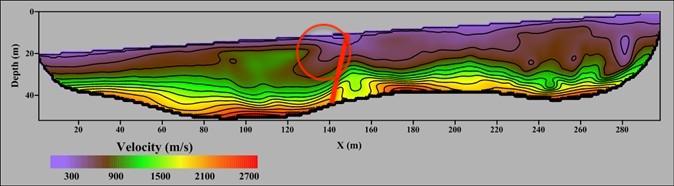
\includegraphics[width=0.9\textwidth]{figures/chap04_field_data/referance_tomo.png} 
               \caption{}
               \label{fig:referance_tomo}
       \end{subfigure}
       \begin{subfigure}[]{1.\textwidth}
               \centering
               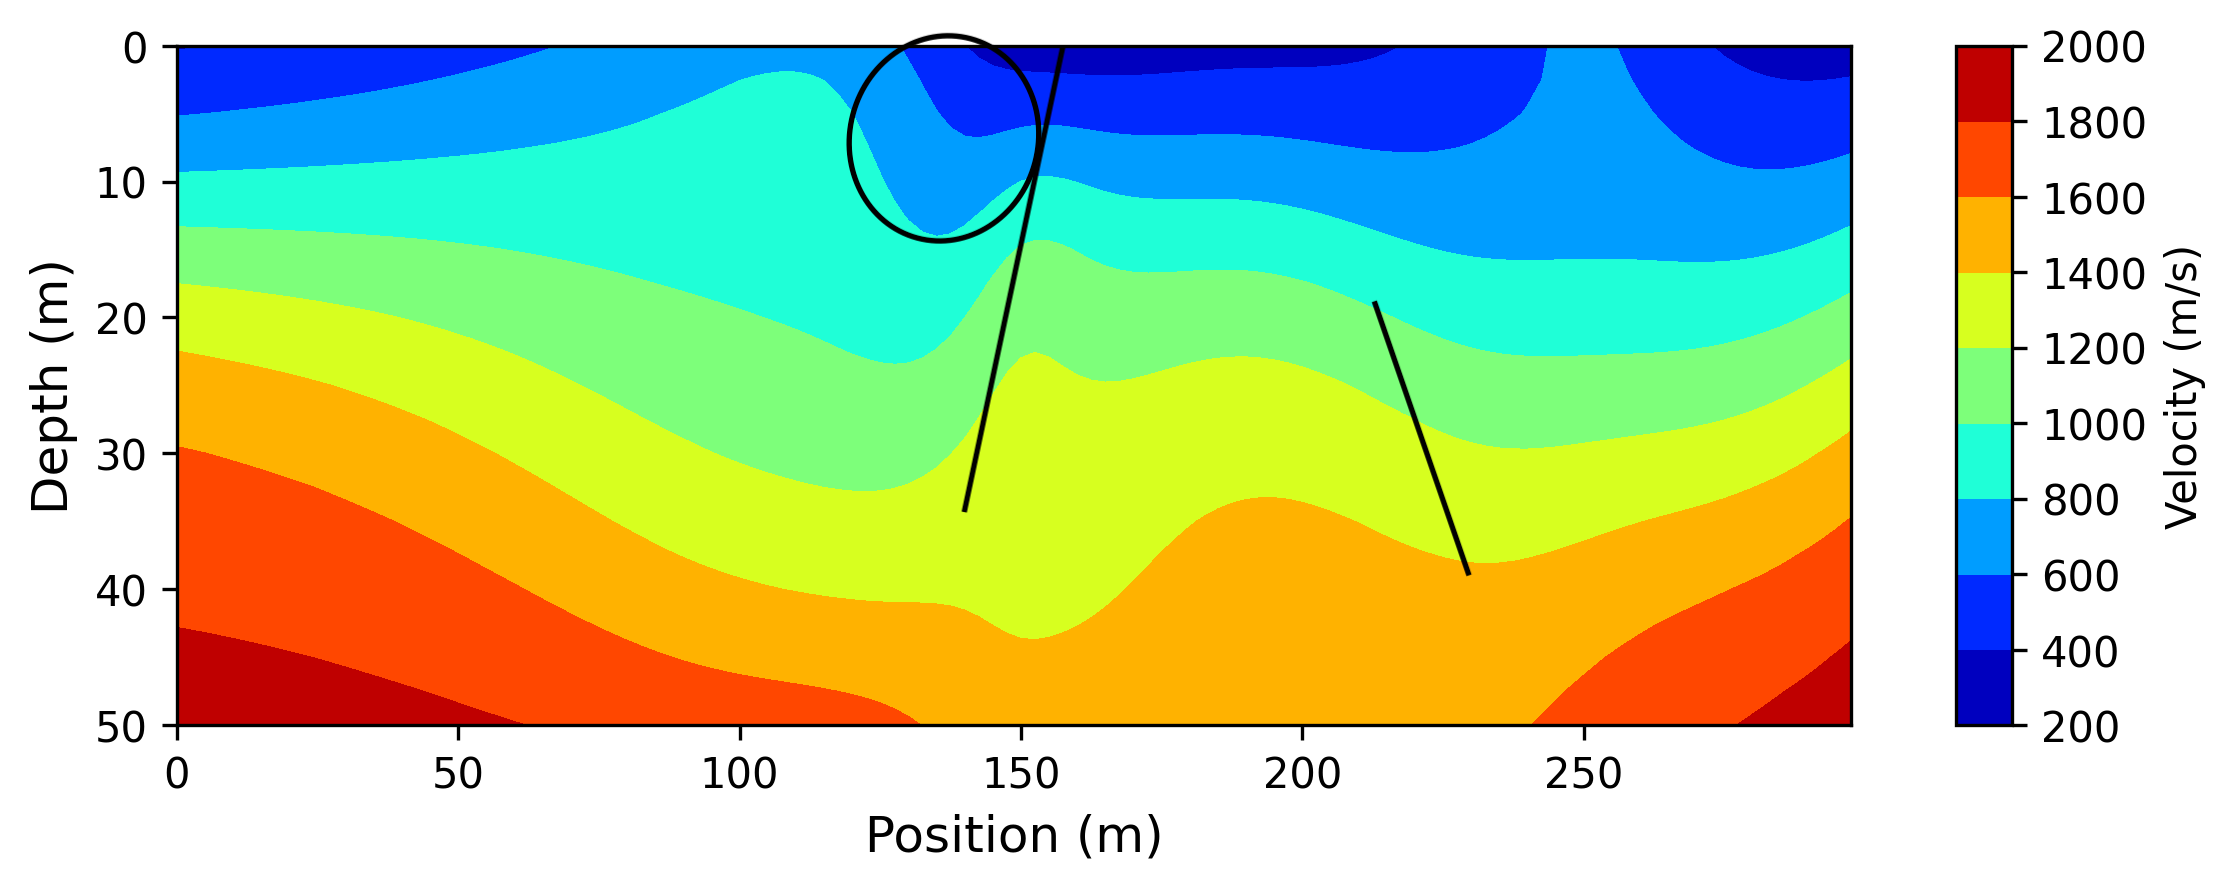
\includegraphics[width=0.9\textwidth]{figures/chap04_field_data/contour_map.png}
               \caption{}
               \label{fig:contour_map}
       \end{subfigure}
       \caption{(a) Traveltime tomogram obtained from a conventional tool (courtesy of Sherif M. Hanafy, King Fahd University of Petroleum and Minerals). The red line marks the interpreted fault location, while the red circle is interpreted as a colluvial wedge.  (b) Contour map representation of the tomogram predicted by PINN. The blacked lines indicate the interpreted faults, while the black circle is interpreted as a low-velocity wedge. }
       \label{fig:comparison}
\end{figure}